\section{Purpose}
\subsection{General Purpose}

The main scope of this document is to define requirements for the application development, in order to make a correct project planification. 
To do this, we will analyze:

\begin{itemize}
\item System;
\item Functional and unfunctional requirements;
\item Constraints;
\item Relationships between stakeholders;
\item Possible scenarios and tests;
\end{itemize}
\medskip
These will be shown using different types of languages, starting from the natural language to the structured languages such as Alloy and UML.
Then, we will define the context in which our application will be developed.
During Sars-Cov-2 emergency, several countries imposed the lockdown in order to hinter the virus diffusion.
People had to change their habits, in fact they could go out only for necessary needs, such as going to the market or pharmacy.
A lot of rules were introduced: not only using the masks or clean your hands but also keeping a social distance.
For instance people must pay attention while they're entering in the market due to the long queue, which could increase the possibility of virus diffusion.
This fact obliged people to stay for a long time standing up and waiting their turn losing a lots of time. 




\subsection{Goals}
\begin{description}
    \item[G1]User enters once arrived at the market
    \item[G2]Put a limit to the number of Users in the market
    \item[G3]Smart User can make a Reservation
    \item[G4]Smart User can make a Visit
    \item[G5]Mobile User can make a Reservation
    \item[G6]Mobile User can make a Visit
    \item[G7]Smart User can cancel a Booking
    \item[G8]Mobile User can cancel a Booking
\end{description}

 
\section{Scope}

The aim of the project is to develop an application which, thanks to an intuitive interface, will avoid a long waiting outside the market.
In order to do that we offer customers three grocery shopping option: 

\begin{itemize}
\item \textbf{Visit}: it's a planned appointment with given date and range time;
\item \textbf{Reservation}: it consits in reserving a virtual seat in market's queue;
\item \textbf{Direct Entrance}: it allows aged customers to enter without any bookings;
\end{itemize}
The main options shown in this documents are the first two in order to avoid customers to line up outside the market. Those are avaiable only for Smart and Mobile Users.
In particular, in order to avoid to wait in line, Users will be allerted by a notification (Smart Users) or a SMS (Mobile Users). These inform them about the own time schedule required to reach the market in time.
Only for Smart User the application will provide the position in queue and the time estimation of the own turn.
Instead a alphanueric string will be provided to Mobile Users due to enter and exit form the market. This string for Smart User is converted in two-dimensional bar code using the standard QRCode. This must be submitted at the entry of the market.
Instead, the third option is only for aged customers older than 65 years old, but with limitations. For instance they can go grocery shopping only in certain days and time slots. 
In particular the Direct Entrance is avaiable only from Monday to Friday in the range time between 9.00 A.M and 13.00 P.M. The reason for this selection is due the fact that in this ranges there are fewer customers than any other periods because are working hours. 




\begin{comment}
The application will provide a QRCode as a virtual ticket on your own smartphone and to wait easily at home or everywhere instead of doing the physical queue for minutes or hours. 
The system will generate a QR code for the authentication at the entry, in order to verify the position in the queue. 
Moreover, the application gives the possibility to "book a visit" for who indicates the approximate expected duration of the visit and how many products they'll buy. \par \medskip
Although the reservation is made entirely with your smartphone, the market gives anyway the possibilities to provide the ticket, acting as proxies for the customers. 
[...]
This is mostly for aged people who are technologically backward or has no smartphone.
Once this procedure is completed, a SMS will be sent to the customers for noticing their turn. [todo]\par \medskip
In order to achieve the goal, we adopt the "World and Machine" model in order to analyse the domain.
\end{comment}



\subsection{World}

It represents the environment in which the system is placed. In particular it's composed by events which are affected by the system,but not directly connected with it.
The main \textit{World Phenomena} are:

\begin{itemize}
\item An User can access to the market;
\item Limit number of Users in the market;
\item User can book his appointment for grocery shopping;
\item User use his mobilephone / smartphone;
\item Respecting social distance;
\end{itemize}

In our application we are going to focus on this World Phenomena excepting for the last one. In fact, during the development of the RASD, we [...]

\subsection{Machine}
It represents the portion of system to be developed.
The main \textit{Machine Phenomena} are:
\begin{itemize}
\item \textit{Internal operations};
\item \textit{Queue menager};
\item \textit{Waiting time estimation};
\item \textit{Data queries};
\end{itemize}
\subsection{Shared Phenomena} 
In this model it needs a common interface to link World and Machine which is composed by the Shared phenomena. Graphically is represent by an intersection between the World and the Machine. In this way World and Machine phenomena are observed from each other.  
The main application Shared Phenomena are the following:

\begin{itemize}
\item \textit{Notifications};
\item \textit{Sign in / Sign up};
\item \textit{Booking management};
\item \textit{QRCode submission};
\item \textit{Appointment request};
\end{itemize}


\section{Definitions, Acronyms, Abbreviations}
\subsection{Definitions}

\begin{itemize}

\item \textbf{Mobilephone}: Elettronic device without CLup App;
\item \textbf{Smartphone}: Elettronic devide with Clup App; 
\item \textbf{CLup App}: It's the application described in this document. It's an application used to make and manage Booking in order to go grocery shopping;
\item \textbf{User}: Generic customer who plan to shop in the market. He could be a Smart or Mobile User;
\item \textbf{Smart User}: User who has got CLup App and so he's able to manage Booking by himself;
\item \textbf{Mobile User}: User who hasn't got CLup App and so he's not able to manage Booking by himself. For instance could be an User who has a dated mobile phone or simply he doesn't install the CLup App. A Mobile User allows a Receptionist to manage his booking by calling a telephone number by interacting with him;
\item \textbf{Shopping Size}: It's the dimensione of the grocery shopping. It could be \textit{Small}, \textit{Medium}, \textit{Large} depending on the number of items that is going to be purchased;  % [S 10, M 20, L 30];
\item \textbf{Booking}: It indicates the generic appointment of a User in the market. It could be a Reservation or a Visit;
\item \textbf{Reservation}: It's a type of Booking. Users simply book a seat at the market's queue. In addition User have to indicate the Shopping Size; 
\item \textbf{Visit}: It's a Booking planned in advance by Users. It is planned by putting the date and the range time in which the User is going grocery shopping. In addition User have to indicate the Shopping Size; 
\item \textbf{Reader}: It reads QRCode at the market's entrance. It allows User to go in;
\item \textbf{Booking submitted}: It means that the QRCode referred to the actual Booking is already submitted in the Reader;
\item \textbf{Visit activated}: It's a Visit which already booked but not yet submitted by the User;
\item \textbf{Reservation activated}: It's a Reservation which already booked but not yet submitted by the User;
\item \textbf{Waiting Time}: It's the time estimated by the system in which, by prevision, an User waits before he enters in the market;
\item \textbf{Shopping Time}: It's the time needed by a User to complete his own grocery shopping;
\item \textbf{Closure Time}: It's the range time in which the market is closed;
\end{itemize}

\begin{comment}


\item \textbf{Delayed ticket}: a ticket is delayed when, after the its ticket call, the user is not submit the QRCode in time (threshold of 1-2 minutes);
\item \textbf{Cancelled ticket}: a ticket is cancelled when it's already delayed and passed too much time (threshold of 15-20 minutes);
\item \textbf{BookingID}: string of n alphanumerical characters that is represented by the QRCode. If the user is not registered [...];


\end{comment}
\begin{itemize}
\subsection{Acronyms}
\item \textbf{RASD}: Requirement Analysis and Specification Document;
\item \textbf{HW}: Hardware;
\item \textbf{SW}: Hardware;
\item \textbf{API}: Application Programming Interface;
\item \textbf{HTTPS}: Hypertext Transfer Protocol Secure;
\item \textbf{DBMS}: Database Management System;

\end{itemize}


\begin{figure}[H]
  \caption{World and Machine rapresentation}
  \label{fig:Reservation}
  \centering
  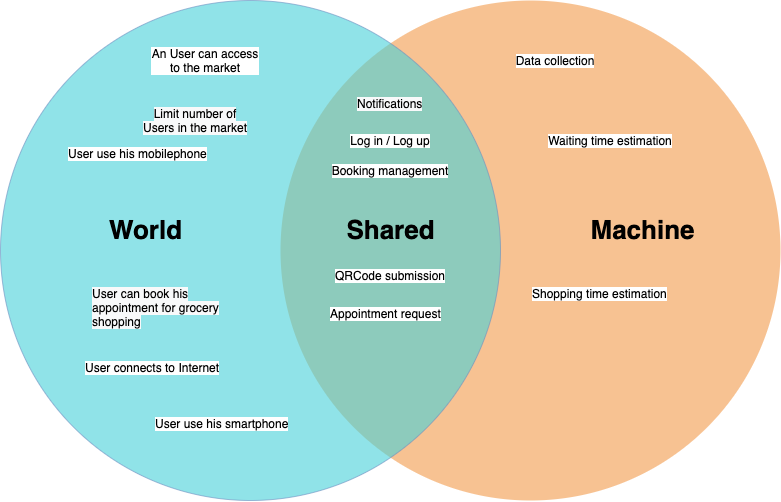
\includegraphics[scale = 0.38]{diagrams/VENN.png}
\end{figure}


\subsection{Abbreviations}
\begin{itemize}
\item \textbf{App}: Application;

\end{itemize}



\section{Revision history}

\section{Reference Documents}
This document is strictly based on:
\begin{itemize}
\item The specification of the \textbf{RASD and DD assignment} of the Software Engineering II corse, held by professor Matteo Rossi and Elisabetta Di Nitto at the Politecnico di Milano, A.Y 2020/2021;
\item \textbf{Slides} of Software Engineering 2 course on BEEP;
\end{itemize}
\section{Document Structure}
Mainly the current document is divided in 4 chapters, which are:
\begin{itemize}
\item[1]\textbf{Introduction}: it aims to describe the environment and the demands taken into account for this project. In particular it's focused on the reasons and the goals that are going to be achieved with its development;
\item[2]\textbf{Overall Description}: it's a high-level description of the system by focusing on the shared phenomena and the domain model (with its assumption). 
\item[3]\textbf{Specific Requirements}: it describes in very detail the requirements needed to reach the goals. In addition it contains more details useful for developers (i.e information about HW and SW interfaces);
\item[4]\textbf{Formal Analysis}: this section contains a formal description of the main aspect of the World phenomena by using Alloy. 
\item[5]\textbf{Effort Spent}: it shows the time spent to realize this document, divided for each section;
\item[6]\textbf{References}: it contains the references to any documents and to the Softwares used in this document.
\end{itemize}

